\documentclass{tufte-handout}

\usepackage{amssymb,amsmath}
% \usepackage{mathspec}
\usepackage{graphicx,grffile}
\usepackage{longtable}
\usepackage{booktabs}
\usepackage{pdfpages}

\newtheorem{mydef}{Definition}[section]
\newtheorem{thm}{Theorem}[section]
\setcounter{section}{4}

\DeclareMathOperator*{\argmin}{arg\,min}
\DeclareMathOperator*{\argmax}{arg\,max}
\newcommand{\Lim}[1]{\raisebox{0.5ex}{\scalebox{0.8}{$\displaystyle \lim_{#1}\;$}}}
\newcommand{\E}{\mathbb{E}}
\newcommand{\Prob}{\mathbb{P}}
\newcommand{\V}{\text{Var}}
\newcommand{\iid}{\stackrel{iid}{\sim}}
\newcommand{\cblack}{\color{Black}}
\newcommand{\cblue}{\color{MidnightBlue}}

\providecommand{\tightlist}{%
  \setlength{\itemsep}{0pt}\setlength{\parskip}{0pt}}

\begin{document}

\justify

{\LARGE Handout 07: Review}

\vspace*{18pt}

\noindent
We have now covered the three key types of tasks that we do in
classical statistics: point estimation, confidence intervals, and
hypothesis tests. We have derived these for the four most common
cases of estimating the mean and variance of one sample as well as
comparing the mean and variance across two samples. Let's review
these concepts in the abstract case of estimating some unknown
parameter $\theta$.

A \textbf{point estimator} is a sample statistic $\hat{\theta}$ 
that is the best guess for the unknown $\theta$. Typically, the
first thing we would want to do is determine the expected value
and variance of $\hat{\theta}$. The quantity
$\mathbb{E}[\hat{\theta}] - \theta$ is called the bias, which
we hope will be close to zero. We say that an estimator is
consistent if both the bias and variance limit to zero in the
limit as the sample size goes to infinity.\footnote{
  I gave the more formal definition on the original handout,
  but this description is equivalent as long as the variance
  is finite.
}

\textbf{Confidence intervals} and \textbf{hypothesis tests}
both require starting by specifying a confidence level $1-\alpha$.
To form either, we typically start by constructing a pivot quantity
$G_\theta$ that is (1) a function of the random sample and the unknown
parameter $\theta$, and (2) has a fixed distribution $\mathcal{G}$
that does not depend on $\theta$. If we let $g_{\alpha}$ be the
critical values of $\mathcal{G}$, we can write the following:
\begin{align*}
\mathbb{P} \left[ g_{1 - \alpha/2} \leq G_\theta \leq g_{\alpha/2} \right] = 1 - \alpha.
\end{align*}
To form a valid confidence interval, we plug in the formula for $G_\theta$
and try to re-arrange to inequality to get the quantity $\theta$ on its
own. In other words, we get:
\begin{align*}
\mathbb{P} \left[ L \leq \theta \leq U \right] = 1 - \alpha.
\end{align*}
And that's exactly what we need. For a hypothesis test, we start with
some null-hypothesis $H_0: \theta = \theta_0$. Given this, we can
compute the actual value $G_{\theta_0}$ given the random sample. We
form the rejection region as follows:
\begin{align*}
R &= \left\{ G_{\theta_0} \leq g_{1-\alpha/2} \right\} \cup \left\{ G_{\theta_0} \geq g_{\alpha/2} \right\}.
\end{align*}
If $G_{\theta_0}$ is in the rejection region, we reject $H_0$; otherwise
we retain the null hypothesis. The $p$-value is defined as the
largest value of $\alpha$ such that $G_{\theta_0}$ is in the rejection
region.\footnote{
  Therefore, for any confidence level where the p-value is less than
  $\alpha$ would result in $G_{\theta_0}$ being within the rejection
  region. 
}
We can compare the $p$-value to our desired $\alpha$ to determine
whether to retain or reject $H_0$.

\vspace*{18pt}

\noindent
Given a point estimator, you should be able to determine its bias and
decide if it is consistent. Given a pivot quantity, you should be able
to construct a confidence interval and set-up an hypothesis test. We
do not know how to do yet is how to produce the point estimators and
pivots in the first place. That will be the focus on the second unit of
the course. 

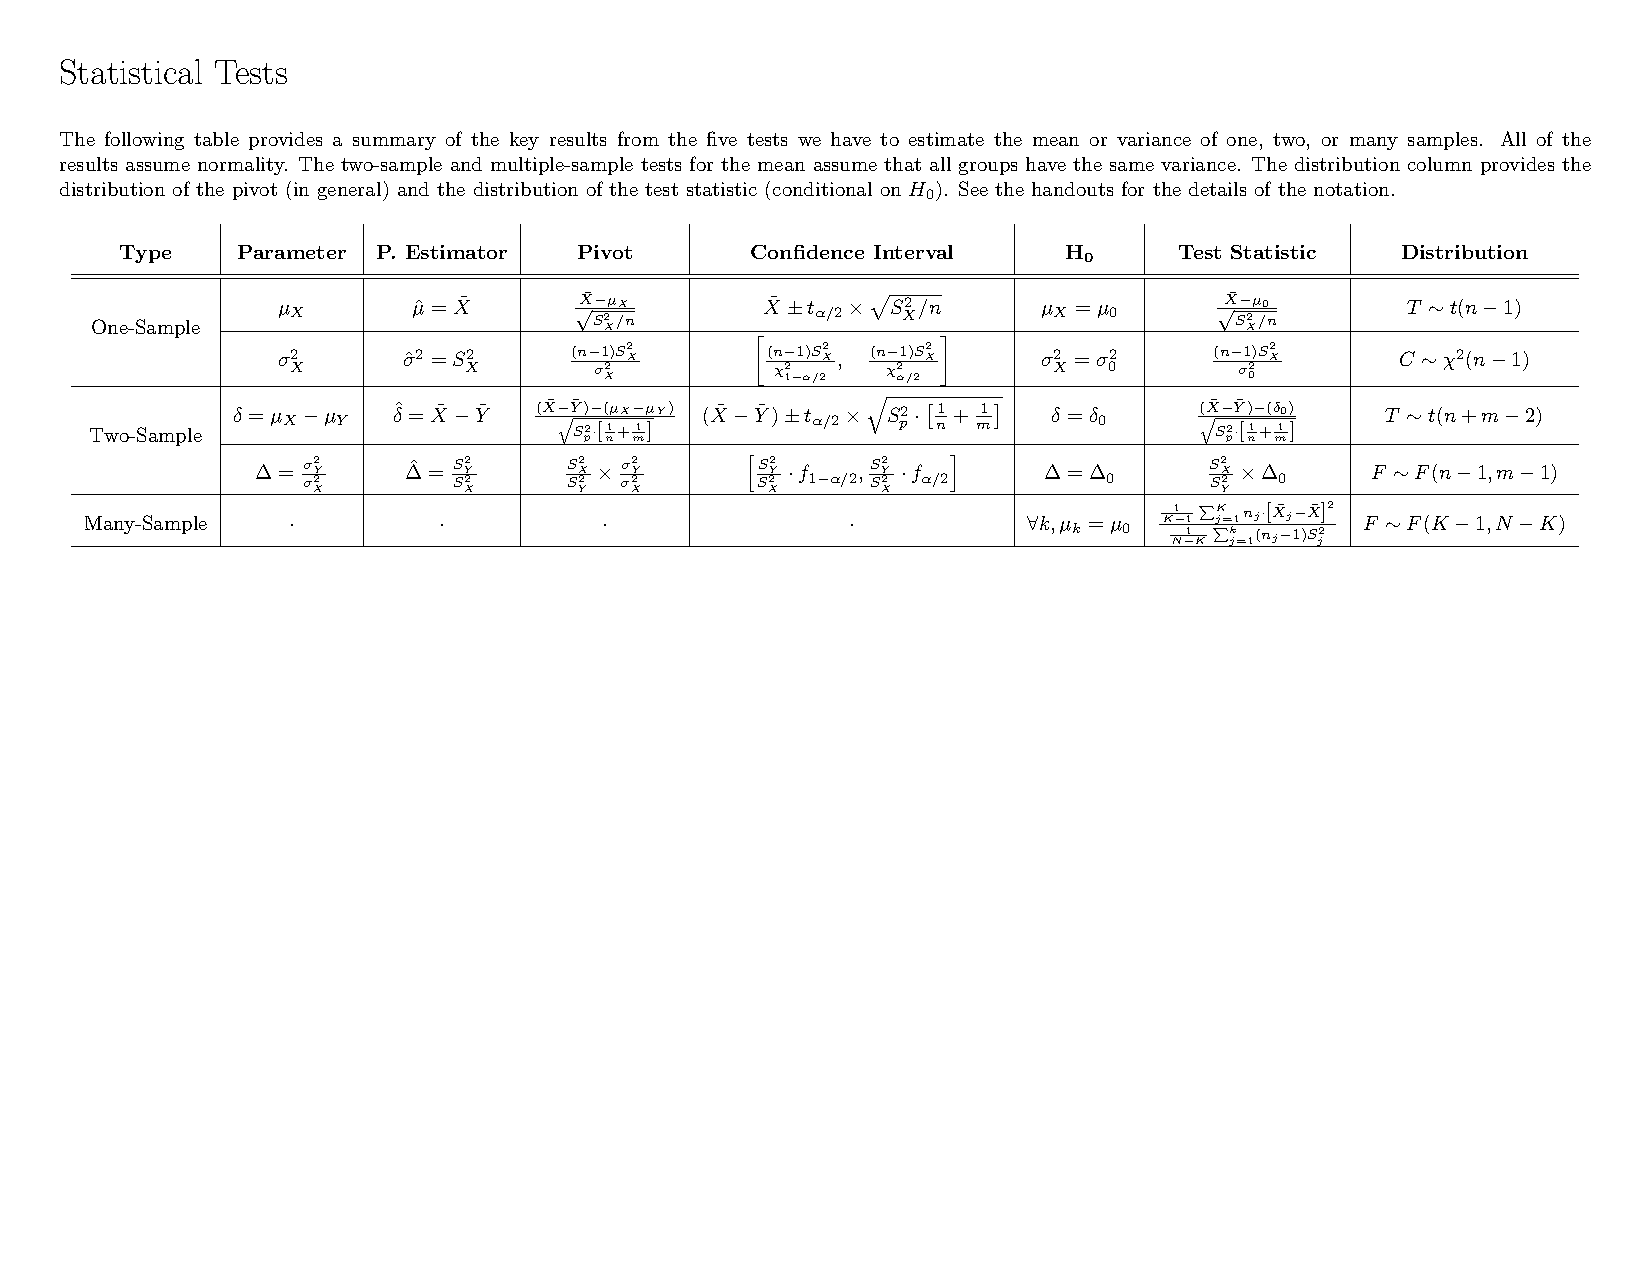
\includepdf[pages=-,landscape]{../extra/tests2}

\end{document}





